\documentclass[a4paper,12pt]{article}

%----------------------- 宏包引入 -----------------------
\usepackage{ctex}       % 中文支持
\usepackage{graphicx}   % 图片支持
\usepackage{geometry}   % 页面布局
\usepackage{listings}   % 代码展示
\usepackage{xcolor}     % 颜色支持
\usepackage{hyperref}   % 超链接
\usepackage{amsmath}    % 数学公式
\usepackage{amssymb}    % 数学符号
\usepackage{booktabs}   % 专业表格
\usepackage{fancyhdr}   % 页眉页脚
\usepackage{lastpage}   % 引用最后一页
\usepackage{caption}    % 标题设置
\usepackage{subfigure}  % 子图支持
\usepackage{float}      % 强制图片位置
\usepackage{enumitem}   % 列表优化
\usepackage{tikz}       % 绘图工具
\usepackage{pgfplots}   % 画折线图
\usepackage{longtable}  % 长表格支持
\usepackage{array}      % 表格增强
\usepackage{multirow}   % 多行单元格
\usepackage{placeins}   % 控制浮动体
\pgfplotsset{width=10cm,compat=1.9}
\usetikzlibrary{shapes,arrows,positioning,automata,calc}

%----------------------- 页面设置 -----------------------
\geometry{left=2.5cm,right=2.5cm,top=2.8cm,bottom=2.8cm}
\linespread{1.5} 
\setlength{\headheight}{14.5pt}

%----------------------- 解决排版问题 -----------------------
\renewcommand{\textfraction}{0.05}
\renewcommand{\topfraction}{0.95}
\renewcommand{\bottomfraction}{0.95}
\renewcommand{\floatpagefraction}{0.8}
\setcounter{topnumber}{3}
\setcounter{bottomnumber}{3}
\setcounter{totalnumber}{5}

%----------------------- 代码高亮设置 -----------------------
\definecolor{codegreen}{rgb}{0,0.6,0}
\definecolor{codegray}{rgb}{0.5,0.5,0.5}
\definecolor{codepurple}{rgb}{0.58,0,0.82}
\definecolor{backcolour}{rgb}{0.97,0.97,0.97}

\lstdefinestyle{mystyle}{
    backgroundcolor=\color{backcolour},   
    commentstyle=\color{codegreen}\itshape,
    keywordstyle=\color{blue}\bfseries,
    numberstyle=\tiny\color{codegray},
    stringstyle=\color{codepurple},
    basicstyle=\ttfamily\small, 
    breakatwhitespace=false,         
    breaklines=true,                 
    captionpos=b,                    
    keepspaces=true,                 
    numbers=left,                    
    numbersep=8pt,                  
    showspaces=false,                
    showstringspaces=false,
    showtabs=false,                  
    tabsize=4,
    frame=shadowbox,
    frameround=tttt,
    xleftmargin=2em,
    xrightmargin=1em,
    language=HTML
}
\lstset{style=mystyle}

%----------------------- 页眉页脚 -----------------------
\pagestyle{fancy}
\lhead{\kaishu 软件工程团队文档}
\chead{需求文档} 
\rhead{第15组} 
\lfoot{}
\cfoot{第 \thepage 页 \ / \ 共 \pageref{LastPage} 页}
\rfoot{}
\renewcommand{\headrulewidth}{0.4pt}

\begin{document}

%----------------------- 封面 -----------------------
\begin{titlepage}
    \begin{center}
        \vspace*{2cm}
        
\includegraphics[width=0.5\textwidth]{NKU.png} \\ 
        \vspace*{2cm}
        {\Huge \bfseries 软件工程团队报告} \\
        \vspace{1.5cm}
        {\Large \bfseries 团队作业1：需求文档} \\
        \vspace{3cm}
        
        \begin{tabular}{l l}
            \Large \textbf{团队组号：} & \Large 15 \\
            \Large \textbf{团队成员：} & \Large 杨雨杭、刘轩麟、尹浩燃、张启鑫、王增哲 \\
            \Large \textbf{学号：} & \Large 2310700、2312289、2313547、2313411、2310708 \\   
            \Large \textbf{指导教师：} & \Large 徐思涵 \\
        \end{tabular}
        
        \vfill
        {\Large \today}
    \end{center}
\end{titlepage}

\newpage
\tableofcontents
\newpage

%----------------------- 正文开始 -----------------------

\section{引言}

\subsection{编写目的}
本文档旨在为“nk推协侦探管理系统”微信小程序的开发全生命周期提供精确的功能边界和性能基准。文档不仅详细阐述了推理协会在日常运营中的核心业务逻辑（如物资流转、解谜互动、积分体系等），还明确了非功能性质量属性，作为后续系统架构设计、数据库建模、单元测试及用户验收的权威技术指引。其目标受众包括开发团队、项目评审人员及社团管理人员。

\subsection{项目背景}
随着南开大学推理协会社团规模的日益扩大，传统的基于人工登记的剧本/书籍借阅、QQ群报名活动、以及零散的线下解谜互动已难以满足高效运营的需求。物资流转不透明、数据统计繁杂、社员活跃度缺乏直观反馈成为制约社团发展的痛点。本项目旨在利用微信开发者工具，构建一个集“推理、竞技、社交、管理”于一体的数字化平台，通过游戏化的机制增强社员粘性。

\subsection{术语与缩写说明}
\begin{itemize}[label=---]
    \item \textbf{Dud}：系统内置的关键词匹配互动机器人，形象为一只名为“u0”的生物。
    \item \textbf{传递中 (In-Transit)}：指物资借阅过程中的关键中间状态，即借阅申请已发起但尚未由管理员完成实物核实。
    \item \textbf{积分 (Credit System)}：分为“总累计积分”（决定排行榜）与“可兑换积分”（用于商城消费），两者逻辑上相互独立；积分来源通过积分流水的来源类型进行区分。
    \item \textbf{事件委托}：用户或管理员发布的互助帖、调查任务或社团官方委托，涉及积分报酬的转移与分配。
\end{itemize}

\subsection{参考文献}
\begin{enumerate}[label={[\arabic*]}]
    \item Ian Sommerville. 软件工程(第10版)[M]. 机械工业出版社, 2018.
    \item Grady Booch, James Rumbaugh, Ivar Jacobson. UML用户指南(第2版)[M]. 人民邮电出版社, 2013.
    \item IEEE Std 830-1998, IEEE Recommended Practice for Software Requirements Specifications[S].
\end{enumerate}

\section{系统概述}

\subsection{系统目标与范围}
本系统旨在构建一个全方位的社团数字化管理闭环。其核心业务范围涵盖以下13个模块：
\begin{itemize}
    \item \textbf{日常互动}：每日谜题解答与解析、Dud关键词自动回复系统。
    \item \textbf{物资管理}：剧本杀与书籍借阅流转、后台物资库存清点系统。
    \item \textbf{激励体系}：动态更新的积分排行榜、独立逻辑的积分兑换商城、个人电子侦探名片。
    \item \textbf{活动与互助}：具备截止时间逻辑的活动报名系统、涉及积分悬赏的事件委托系统。
    \item \textbf{基础支撑}：账号注册与登录、系统设置、权限控制和通知偏好等常规小程序功能。
\end{itemize}

\subsection{用户角色定义}
系统通过 OpenID 进行身份识别；在数据库字段中统一使用小写 \texttt{openid}，业务描述中统一使用 OpenID。系统主要划分三类角色：
\begin{itemize}
    \item \textbf{未登录用户（游客）}：可浏览不依赖 user\_id 的公开内容，如游戏与书籍推荐、公开活动通知、首页基础信息等；不能参与每日谜题答题、活动报名、积分兑换、物品借阅、事件委托发布、个人名片修改等需要身份绑定的操作。
    \item \textbf{普通用户（侦探）}：拥有答题、查看排名、报名活动、发布/领取委托、借阅申请、商城兑换及个人信息修改权限。
    \item \textbf{管理员（社团管理层）}：除上述权限外，拥有独立的后端控制面板。职责包括物资流转状态的最终确认（将“传递中”转为“借出”）、每日谜题的预设与更新频率控制、库存数据增删改、回复规则的实时配置，以及不定期发布来自社团的官方事件委托。
\end{itemize}

\subsection{系统运行环境}
\begin{itemize}
    \item \textbf{开发环境}：Windows操作系统下的微信开发者工具（Stable Build），利用其内置的WXML、WXSS、JavaScript框架进行敏捷开发。
    \item \textbf{硬件环境}：
        \begin{itemize}
            \item \textbf{开发侧}：运行微信开发者工具的PC设备，利用开发者工具自带的“手机模拟器”进行各种主流分辨率（如iPhone 13/Pro, Android Pixel 5等）的视口效果预览、布局适配及逻辑调试。
            \item \textbf{运行侧}：支持微信客户端运行的移动端智能终端（iOS 10.0 或更高版本；Android 5.0 或更高版本）。
        \end{itemize}
    \item \textbf{网络环境}：稳定的互联网接入，用于云端数据库的数据存取与多端数据同步。
    \item \textbf{后端服务}：微信小程序云开发（或自建云服务器），提供云函数、云数据库、云存储等基础设施。云函数基于Node.js或Python运行时实现业务逻辑与权限管理。
    \item \textbf{支撑工具}：
        \begin{itemize}
            \item Git版本控制系统（托管在GitHub/GitLab，便于团队协作）。
            \item WeChat公众平台与小程序后台（用于配置AppID、AppSecret、消息推送等）。
        \end{itemize}
\end{itemize}

\subsubsection{兼容性要求}
\begin{itemize}
    \item 支持iOS、Android及Web端微信客户端。
    \item 对于低端安卓机型（内存 < 1GB），系统应启用"轻量级模式"，减少动画与图片加载，确保基础功能可用。
    \item 支持离线缓存：用户在没有网络连接时，本地缓存应能显示上次同步的数据，待网络恢复后自动同步。
\end{itemize}

\section{功能性需求}
\label{3}
本章依据原始需求说明、系统用例图、概念类图、关键活动图与状态机图，对“nk推协侦探管理系统”的功能性需求进行细化。系统面向未登录用户（游客）、普通用户（侦探）与管理员（社团管理层）三类角色：未登录用户仅浏览公开内容；普通用户主要完成答题、报名、借阅、兑换、发帖和个人信息维护；管理员在继承普通用户能力的基础上，负责谜题、规则、库存、活动、借阅状态、反馈信息和官方委托的维护。

\begin{figure}[H]
    \centering
    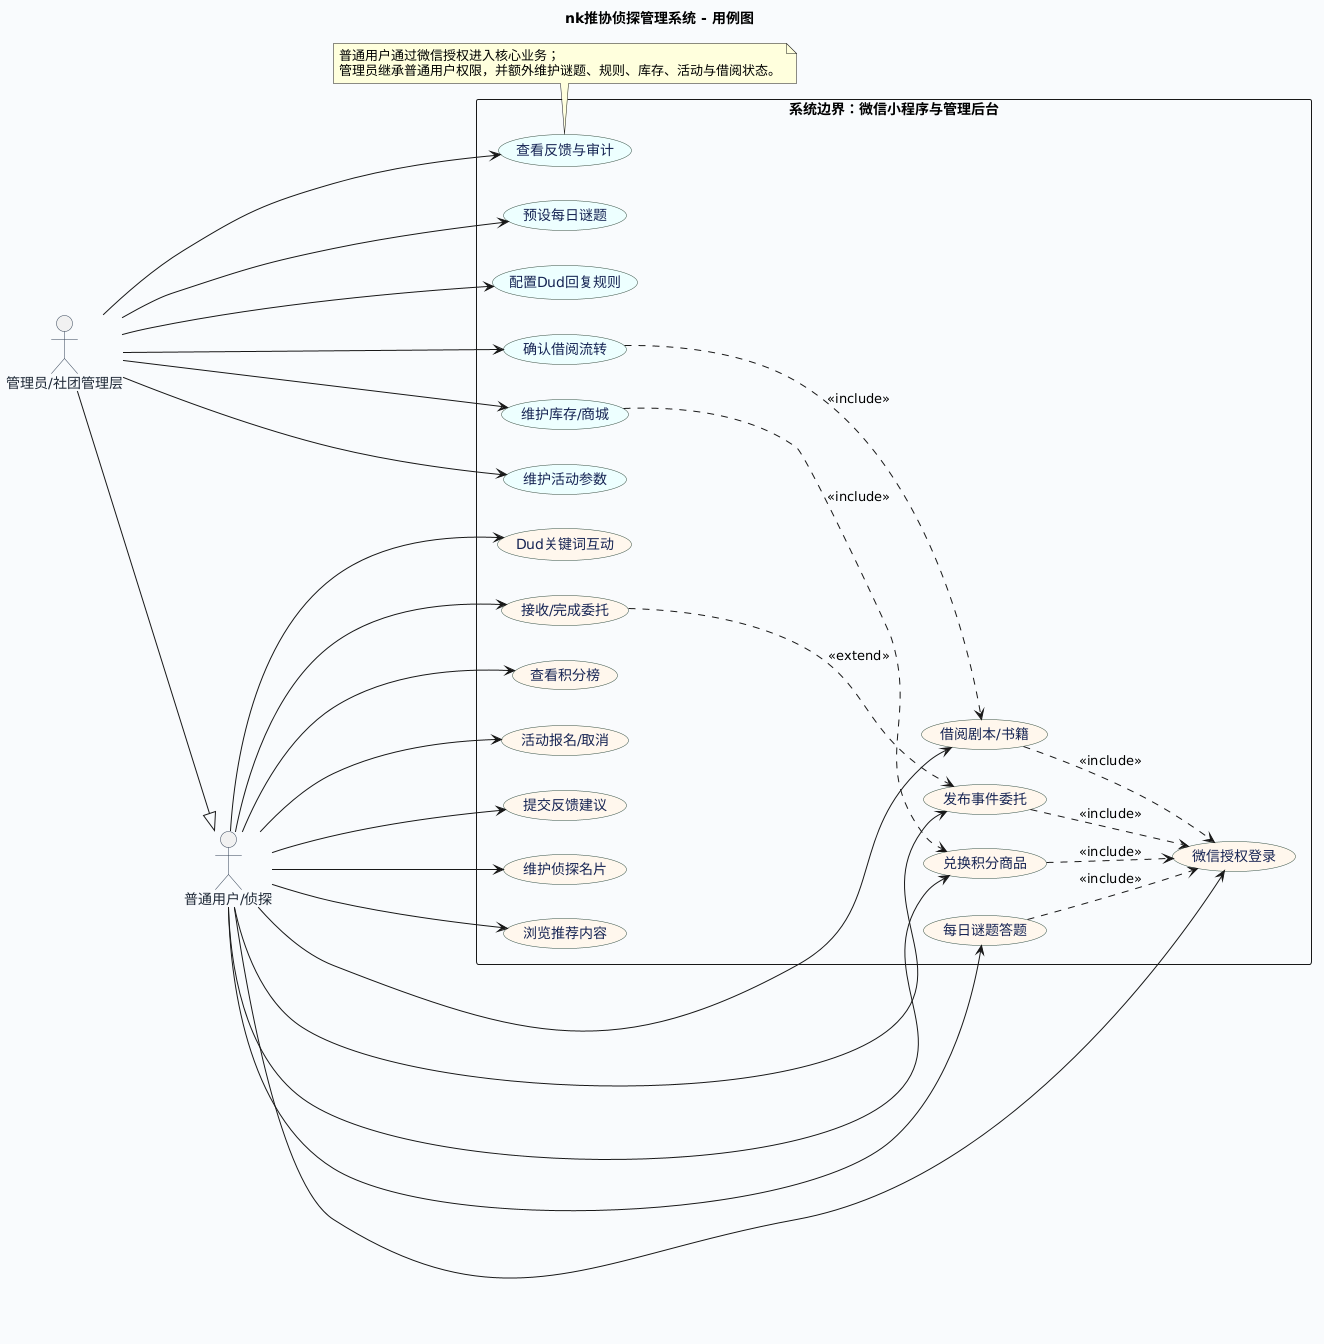
\includegraphics[width=0.78\textwidth,height=0.68\textheight,keepaspectratio]{uml_output/use_case_diagram.png}
    \caption{系统用例图}
    \label{fig:use-case-diagram}
\end{figure}

如图 \ref{fig:use-case-diagram} 所示，系统核心用例可分为日常互动、积分激励、活动互助、物资管理和后台维护五类。各用例之间以“微信授权登录”为权限入口，以“积分账户”和“库存管理”为共享业务基础。

\begin{figure}[H]
    \centering
    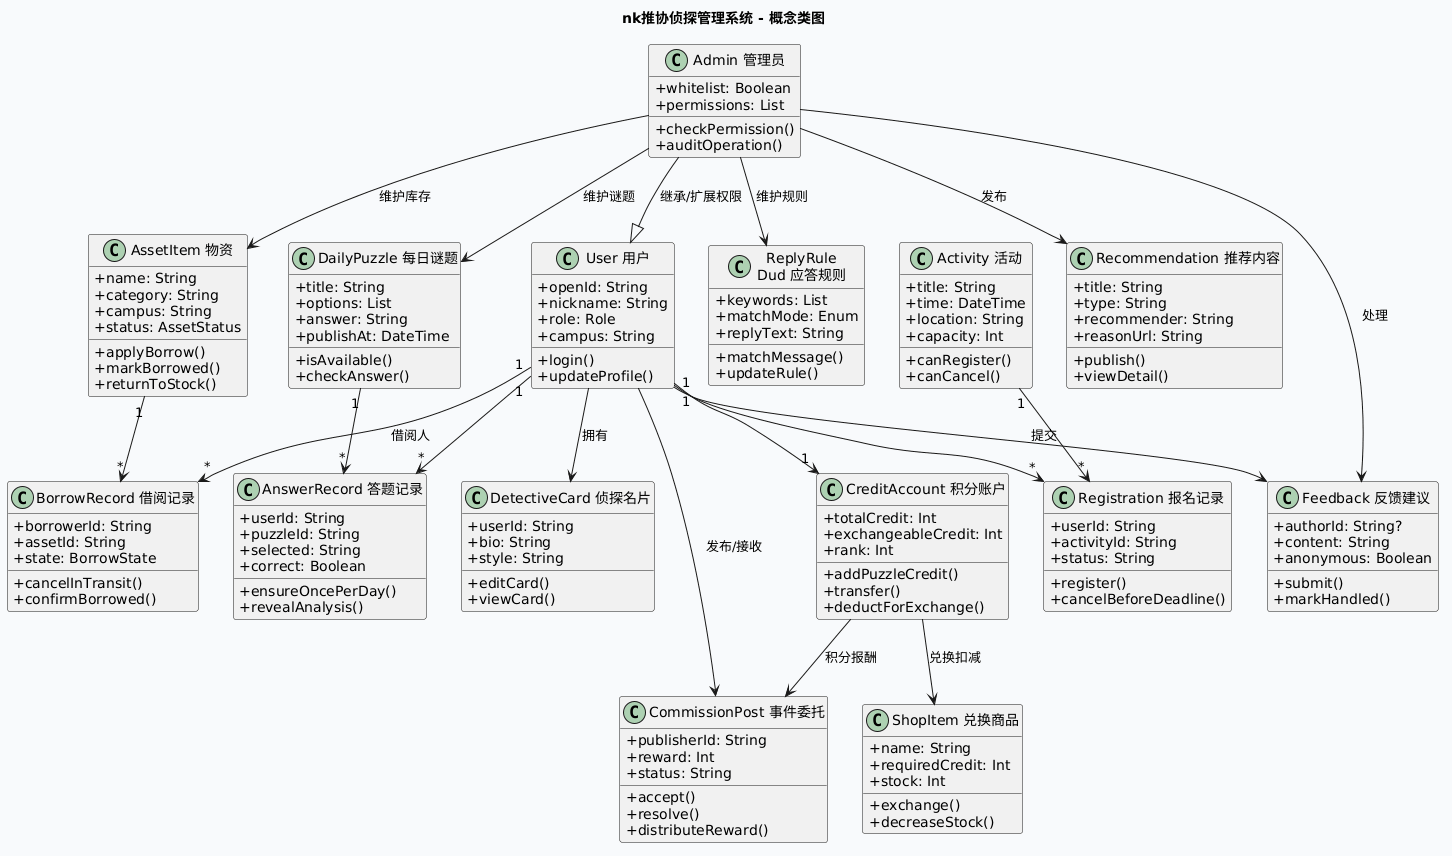
\includegraphics[width=0.9\textwidth,height=0.62\textheight,keepaspectratio]{uml_output/class_diagram.png}
    \caption{系统概念类图}
    \label{fig:class-diagram}
\end{figure}

图 \ref{fig:class-diagram} 展示了功能需求对应的主要业务对象，包括用户、管理员、每日谜题、答题记录、积分账户、活动、物资、借阅记录、Dud回复规则、事件委托、反馈建议和推荐内容。后续需求描述均以这些对象及其关系为基础。

\subsection{用例总览}

{\small
\setlength{\tabcolsep}{3pt}
\begin{longtable}{>{\raggedright\arraybackslash}p{0.10\textwidth}>{\raggedright\arraybackslash}p{0.18\textwidth}>{\raggedright\arraybackslash}p{0.17\textwidth}>{\raggedright\arraybackslash}p{0.37\textwidth}}
    \caption{系统主要用例概览}
    \label{tab:use-case-summary}\\
    \toprule
    用例编号 & 用例名称 & 参与者 & 目标说明 \\
    \midrule
    UC-01 & 微信授权登录 & 普通用户、管理员 & 通过 OpenID 识别身份，建立有效会话，并区分普通用户与管理员权限；数据库字段统一保存为 \texttt{openid}。 \\
    UC-02 & 每日谜题答题 & 普通用户 & 用户每日完成一次谜题作答，系统根据结果展示答案解析并更新积分。 \\
    UC-03 & 查看积分榜 & 普通用户 & 用户查看首页前三名、完整前100名榜单及个人实时排名。 \\
    UC-04 & 积分兑换商品 & 普通用户 & 用户使用可兑换积分兑换奖品，系统扣减可兑换积分与商城库存。 \\
    UC-05 & 活动报名/取消 & 普通用户、管理员 & 用户报名或取消活动；管理员维护活动时间、地点、人数上限与取消截止时间。 \\
    UC-06 & 借阅剧本/书籍 & 普通用户、管理员 & 用户申请借阅社团物资，管理员确认实物交接并维护物资状态。 \\
    UC-07 & Dud关键词互动 & 普通用户、管理员 & 用户在对话界面输入内容，Dud按关键词规则回复；管理员维护回复规则。 \\
    UC-08 & 浏览推荐内容 & 普通用户、管理员 & 用户浏览游戏/书籍推荐；管理员发布和维护推荐内容。 \\
    UC-09 & 维护侦探名片 & 普通用户 & 用户编辑个人资料、积分展示与名片样式，并在社交场景中对外展示。 \\
    UC-10 & 事件委托/调查 & 普通用户、管理员 & 用户发布求助任务、接收委托、确认完成并分配积分报酬；管理员可发布来自社团的官方委托。 \\
    UC-11 & 提交反馈建议 & 普通用户、管理员 & 用户提交反馈或活动建议；管理员查看、标记和处理反馈。 \\
    UC-12 & 库存管理 & 管理员 & 管理员维护书籍、剧本杀、兑换商品和社团杂物的库存信息。 \\
    UC-13 & 账号注册与登录 & 未登录用户、普通用户、管理员 & 未登录用户可浏览公开内容，授权后创建账号并获得需要 user\_id 的操作权限。 \\
    UC-14 & 系统设置 & 普通用户、管理员 & 用户维护通知、隐私和登录状态等设置；管理员维护系统级参数。 \\
    \bottomrule
\end{longtable}
}

\subsection{每日谜题系统}

\subsubsection{基本描述}
每日谜题是系统的核心互动入口，用于提高社员日常参与度并产生积分数据。系统每日在预设时间点更新谜题，每名已登录用户每天仅有一次作答机会。每日谜题流程如图 \ref{fig:activity-daily-puzzle} 所示。

\begin{figure}[H]
    \centering
    \begin{minipage}[c]{0.34\textwidth}
        \centering
        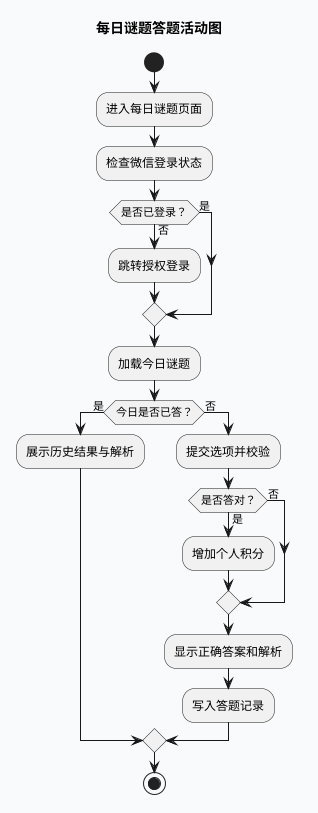
\includegraphics[height=0.42\textheight,keepaspectratio]{uml_output/activity_daily_puzzle.png}
    \end{minipage}
    \hfill
    \begin{minipage}[c]{0.56\textwidth}
        \small
        \textbf{流程要点：}
        \begin{itemize}[leftmargin=1.4em,itemsep=0.2em]
            \item 进入页面后先校验微信登录状态，未登录用户需完成授权。
            \item 系统加载当日谜题，并判断用户今日是否已经提交答案。
            \item 未答用户提交选项后立即得到答案与解析；答对时同步增加积分。
            \item 已答用户再次进入页面时，只展示历史结果与解析，不允许重复提交。
        \end{itemize}
    \end{minipage}
    \caption{每日谜题答题活动图}
    \label{fig:activity-daily-puzzle}
\end{figure}

\subsubsection{功能需求}
\begin{itemize}
    \item \textbf{谜题入口}：首页提供每日谜题入口，但不直接展示额外谜题内容；按钮颜色应根据用户当日是否已答动态变化，待答状态显示为醒目颜色，已答状态显示为灰色或弱化样式。
    \item \textbf{登录校验}：仅已完成微信授权登录的用户可以提交答案。未登录用户进入谜题页时，系统应引导其完成授权。
    \item \textbf{谜题更新}：管理员可在后台预先设置谜题、选项、正确答案、解析与发布时间。系统到达发布时间后自动切换当日谜题。
    \item \textbf{选项支持}：每道谜题允许设置不等数量的选项，系统不得将选项数量固定为某一常量。
    \item \textbf{答题限制}：同一账号每天只能提交一次答案。提交限制必须在前端与后端同时校验。
    \item \textbf{答案反馈}：用户提交答案后，系统应立即展示正确答案和解析，无论用户是否答对。
    \item \textbf{积分奖励}：用户答对后，系统应同时增加“总累计积分”和“可兑换积分”；用户答错时不增加积分，但仍记录作答结果。
\end{itemize}

\subsection{积分排行榜}

\subsubsection{基本描述}
积分排行榜用于展示用户在积分方面的竞争排名。排行榜以“总累计积分”为排序依据，不区分积分来源，具体来源在积分流水类型中记录，且不受商城兑换和委托支出影响。

\subsubsection{功能需求}
\begin{itemize}
    \item \textbf{首页预览}：首页仅显示排行榜前三名，包括昵称、头像或标识、积分数和排名。
    \item \textbf{完整榜单}：用户点击首页入口后进入排行榜页面，页面最多展示前100名用户，并同时显示排名与积分。
    \item \textbf{更新频率}：排行榜可按每日更新，更新时间点应与每日谜题结算或谜题更新时间保持一致。
    \item \textbf{个人排名}：个人页面应显示用户实时总积分与当前排名。若用户未进入前100名，应显示“未入榜”。
    \item \textbf{并列处理}：若第100名附近存在多名用户积分相同，系统应额外显示并列排名信息，避免用户因截断规则无法确认自身位置。
    \item \textbf{个人高亮}：当当前用户位于排行榜前100名时，榜单中该行应使用额外颜色标注。
\end{itemize}

\subsection{积分兑换商城}

\subsubsection{基本描述}
积分兑换商城用于将用户活跃度转化为可感知奖励。商城只扣减“可兑换积分”，不得扣减用于排行榜的“总累计积分”。

\subsubsection{功能需求}
\begin{itemize}
    \item \textbf{商品展示}：商城页面应展示可兑换奖品名称、图片或说明、所需积分和剩余库存。
    \item \textbf{积分校验}：用户点击兑换时，系统应校验其可兑换积分是否充足；不足时提示兑换失败原因。
    \item \textbf{兑换扣减}：兑换成功后，系统仅扣减用户可兑换积分，并保持总累计积分不变。
    \item \textbf{库存同步}：商城商品库存应与后台库存管理系统使用同一数据源，兑换成功后即时扣减库存。
    \item \textbf{兑换记录}：系统应记录兑换时间、商品、消耗积分、处理状态，并在用户个人页面展示历史记录。
\end{itemize}

\subsection{活动通知与报名系统}

\subsubsection{基本描述}
活动系统用于发布社团近期活动并管理报名流程。活动按时间顺序展示，用户可报名或在允许时间内取消报名。

\subsubsection{功能需求}
\begin{itemize}
    \item \textbf{活动列表}：系统应提供独立活动页面，按活动时间升序展示近期活动。
    \item \textbf{活动信息}：每个活动至少展示标题、简介、时间、地点、人数上限、当前报名人数和是否报满。
    \item \textbf{报名操作}：未报名用户可点击报名；报名成功后，页面应实时显示“已报名”状态。
    \item \textbf{取消操作}：管理员可为活动设置最晚取消时间。用户在该时间前可取消报名；超过该时间后，取消按钮不可用或操作后弹窗说明原因。
    \item \textbf{不可取消提醒}：若用户在最晚取消时间之后报名，系统必须额外弹窗提醒“当前活动报名后不可取消”，用户确认后方可完成报名。
    \item \textbf{人数上限}：活动达到人数上限后，未报名用户不可继续报名；已报名用户的取消规则仍按截止时间执行。
    \item \textbf{后台维护}：管理员可新增、修改、下架活动，并维护活动容量、地点和截止时间等参数。
\end{itemize}

\subsection{活动申请与反馈建议}

\subsubsection{基本描述}
反馈建议模块为普通用户向管理层提交活动申请、系统问题和社团建议提供入口，相当于面向管理层的留言板。

\subsubsection{功能需求}
\begin{itemize}
    \item \textbf{反馈入口}：首页或个人页面应提供“反馈/建议”入口。
    \item \textbf{文本提交}：用户进入反馈界面后，可输入文本内容并提交。
    \item \textbf{匿名反馈}：系统应支持匿名提交选项；匿名反馈在普通管理视图中不展示用户身份。
    \item \textbf{后台处理}：管理员可查看反馈列表，对反馈进行分类、标记处理状态和记录处理结果。
\end{itemize}

\subsection{剧本杀与书籍借阅系统}

\subsubsection{基本描述}
借阅系统用于展示和流转社团书籍、剧本杀等可借物资。系统需要精确维护“在库”“传递中”“已借出”等状态，避免同一物资被重复借阅。借阅活动流程与核心状态机见图 \ref{fig:borrow-flow-state}。

\begin{figure}[H]
    \centering
    \subfigure[借阅流程活动图\label{fig:activity-borrow}]{
        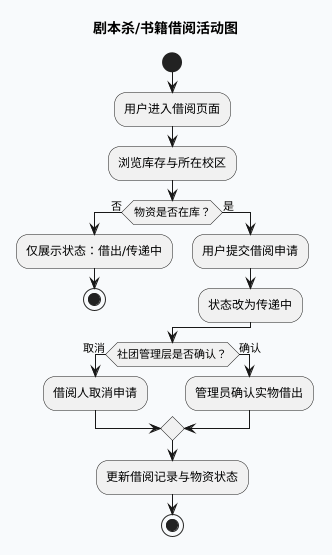
\includegraphics[width=0.42\textwidth,height=0.42\textheight,keepaspectratio]{uml_output/activity_borrow.png}
    }
    \hfill
    \subfigure[借阅物资状态机图\label{fig:state-borrow-asset}]{
        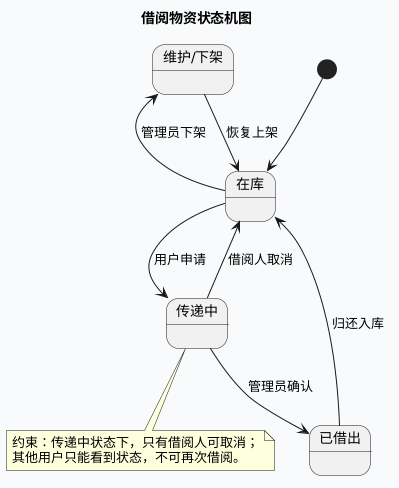
\includegraphics[width=0.45\textwidth,height=0.42\textheight,keepaspectratio]{uml_output/state_borrow_asset.png}
    }
    \caption{借阅流程与物资状态图}
    \label{fig:borrow-flow-state}
\end{figure}

\subsubsection{功能需求}
\begin{itemize}
    \item \textbf{借阅页面}：系统应提供独立借阅页面，根据社团库存展示现有书籍和剧本杀。
    \item \textbf{书籍信息}：书籍条目应显示名称、简介、状态、所在校区和具体存放位置。
    \item \textbf{剧本杀信息}：剧本杀条目除基础信息外，还应显示类型、推荐人数和游玩时长。
    \item \textbf{状态展示}：物资在库时显示可借阅；已借出时显示借出；传递中时显示传递中。
    \item \textbf{借阅申请}：用户确认借阅后，系统应立即将物资状态由“在库”改为“传递中”，并记录借阅人。
    \item \textbf{管理员确认}：社团管理层在实际完成物资交接后，可在后台将状态由“传递中”改为“已借出”。
    \item \textbf{传递中取消}：当物资处于“传递中”时，只有借阅人可以看到并使用“取消”按钮；取消后物资恢复为“在库”。
    \item \textbf{并发限制}：其他用户在“传递中”或“已借出”状态下不可再次借阅该物资。
    \item \textbf{归还入库}：管理员确认归还后，系统应将物资状态由“已借出”改回“在库”，并关闭对应借阅记录。
\end{itemize}

\subsection{游戏与书籍推荐系统}

\subsubsection{基本描述}
推荐系统用于发布游戏、书籍或相关推理内容，为社团成员提供内容发现入口。

\subsubsection{功能需求}
\begin{itemize}
    \item \textbf{首页入口}：首页提供推荐内容入口，点击后进入独立推荐页面。
    \item \textbf{列表浏览}：推荐页面支持上下滑动浏览所有推荐内容。
    \item \textbf{详情弹窗}：用户点击单条推荐后，系统弹窗展示名称、类型、推荐人和推荐理由。
    \item \textbf{外链理由}：推荐理由可表现为跳转公众号文章的按钮，用户点击后进入对应文章或说明页。
    \item \textbf{后台发布}：管理员可新增、修改、隐藏推荐内容，并维护推荐理由链接。
\end{itemize}

\subsection{Dud关键词回复系统}

\subsubsection{基本描述}
Dud关键词回复系统是首页“神秘按钮”对应的互动功能。用户进入独立对话界面后，与名为“u0”的Dud进行关键词匹配式对话。

\subsubsection{功能需求}
\begin{itemize}
    \item \textbf{独立界面}：首页提供神秘按钮入口，点击后进入Dud对话页面。
    \item \textbf{对话展示}：页面应以聊天气泡形式展示用户输入和Dud回复。
    \item \textbf{全匹配规则}：当用户输入与规则关键词完全一致时，系统返回对应回复。
    \item \textbf{半匹配规则}：当用户输入中包含某些关键词时，系统可按半匹配规则返回回复。
    \item \textbf{多关键词规则}：系统应参考公众号多关键词机制，支持同一回复规则下配置多个触发词。
    \item \textbf{默认回复}：若输入未匹配任何规则，系统应返回默认提示。
    \item \textbf{规则维护}：管理员可在后台实时添加、修改、删除回复规则，无需重新发布小程序。
\end{itemize}

\subsection{侦探个人名片系统}

\subsubsection{基本描述}
侦探个人名片是用户注册后的个人展示页面，用于承载积分、排名和基础社交信息，并可在帖子评论区等场景中被他人查看。

\subsubsection{功能需求}
\begin{itemize}
    \item \textbf{信息展示}：个人名片应展示用户昵称、头像、简介、总积分、可兑换积分和当前排名。
    \item \textbf{未入榜提示}：当用户未进入排行榜前100名时，排名字段显示“未入榜”。
    \item \textbf{资料编辑}：用户可修改基础交友信息和个人简介。
    \item \textbf{样式编辑}：用户可调整个人名片设计，例如背景、主题色或展示模板。
    \item \textbf{场景跳转}：在帖子评论区、排行榜、活动报名列表等页面，点击头像可查看对应用户的个人名片。
\end{itemize}

\subsection{事件委托与调查系统}

\subsubsection{基本描述}
事件委托系统提供类似集市发帖/求助的功能。发帖人可消耗可兑换积分作为报酬，其他用户接收委托并在完成后获得积分。管理员也可不定期发布来自社团的官方事件委托，相当于在每日谜题、活动等机制之外，为用户提供一条官方积分获取途径。事件委托流程如图 \ref{fig:activity-commission} 所示。

\begin{figure}[H]
    \centering
    \begin{minipage}[c]{0.32\textwidth}
        \centering
        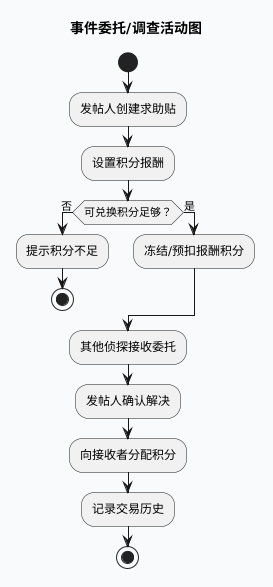
\includegraphics[height=0.38\textheight,keepaspectratio]{uml_output/activity_commission.png}
    \end{minipage}
    \hfill
    \begin{minipage}[c]{0.58\textwidth}
        \small
        \textbf{流程要点：}
        \begin{itemize}[leftmargin=1.4em,itemsep=0.2em]
            \item 发帖人创建求助帖并设置积分报酬。
            \item 系统校验可兑换积分，积分不足时直接阻止发布。
            \item 管理员可发布社团官方委托，奖励来源标记为社团奖励。
            \item 报酬积分在发布时冻结或预扣，避免完成后无法支付。
            \item 委托完成后由发帖人确认分配，系统记录积分流水与交易历史。
        \end{itemize}
    \end{minipage}
    \caption{事件委托活动图}
    \label{fig:activity-commission}
\end{figure}

\subsubsection{功能需求}
\begin{itemize}
    \item \textbf{独立页面}：系统应提供事件委托页面，展示求助帖、悬赏任务和任务状态。
    \item \textbf{发布委托}：用户发布求助贴时，可设置标题、描述、报酬积分和可接收人数等信息。
    \item \textbf{报酬扣减}：发布需要报酬的委托时，系统应校验发帖人可兑换积分是否足够；足够时冻结或预扣对应积分。
    \item \textbf{官方委托}：管理员可代表社团发布官方事件委托，并设置积分奖励、截止时间和审核规则。官方委托的积分来源标记为社团奖励，不从普通用户账户扣除。
    \item \textbf{接收委托}：其他用户可选择接收委托，系统记录接收者与接收时间。
    \item \textbf{完成确认}：发帖人确认事件解决后，可将报酬积分分配给一个或多个接收者。
    \item \textbf{积分转移}：委托完成后，系统将积分转移给接收者，并写入积分流水；总累计积分不因支出而减少。
    \item \textbf{历史记录}：用户可查看自己发布、接收和完成的委托记录。
\end{itemize}

\subsection{库存管理系统}

\subsubsection{基本描述}
库存管理系统仅对管理员开放，用于维护社团物资清点数据。它同时支撑借阅系统和积分兑换商城，是物资状态与库存数量的统一数据来源。

\subsubsection{功能需求}
\begin{itemize}
    \item \textbf{访问权限}：仅管理员可进入库存管理后台，普通用户不得访问。
    \item \textbf{物资分类}：库存应支持书籍、剧本杀、兑换奖品、海报、办公用具等分类。
    \item \textbf{信息维护}：管理员可新增、修改、删除和查询物资信息，包括名称、类别、库存数量、所在校区、具体位置、状态和备注。
    \item \textbf{库存联动}：借阅导致的状态变化和商城兑换导致的数量扣减，必须实时同步到库存管理系统。
    \item \textbf{清点辅助}：管理员可按分类或位置筛选物资，并导出或查看库存清点结果。
\end{itemize}

\subsection{账号注册与登录系统}

\subsubsection{基本描述}
账号注册与登录系统用于建立用户身份、绑定 OpenID 并维护会话状态，是所有需要 user\_id 的业务操作的前置条件。

\subsubsection{功能需求}
\begin{itemize}
    \item \textbf{游客浏览}：未登录用户可浏览游戏与书籍推荐、公开活动通知、首页基础信息等公开内容。
    \item \textbf{注册登录}：用户首次授权登录时，系统应创建用户记录并绑定 OpenID；数据库字段统一保存为 \texttt{openid}。
    \item \textbf{会话维护}：登录成功后系统应建立有效 session，并在会话过期时引导用户重新登录。
    \item \textbf{权限拦截}：每日谜题答题、活动报名、积分兑换、物品借阅、事件委托发布、个人名片修改等操作必须校验登录状态。
    \item \textbf{账号资料}：用户可维护昵称、头像等基础资料，敏感身份标识不得在客户端明文展示。
\end{itemize}

\subsection{系统设置}

\subsubsection{基本描述}
系统设置模块用于集中管理小程序的常规偏好、通知开关和基础运行配置，提升用户使用体验和管理员维护效率。

\subsubsection{功能需求}
\begin{itemize}
    \item \textbf{个人设置}：用户可调整通知提醒、隐私展示、缓存清理和基础界面偏好。
    \item \textbf{通知设置}：支持每日谜题提醒、活动报名提醒、借阅状态提醒、委托进度提醒等开关。
    \item \textbf{安全设置}：用户可查看登录状态并退出登录；系统应清理本地会话缓存。
    \item \textbf{后台设置}：管理员可配置谜题更新时间、活动默认截止规则、积分奖励参数、推荐内容展示开关等系统级参数。
\end{itemize}

\subsection{功能模块依赖}

\begin{figure}[H]
    \centering
    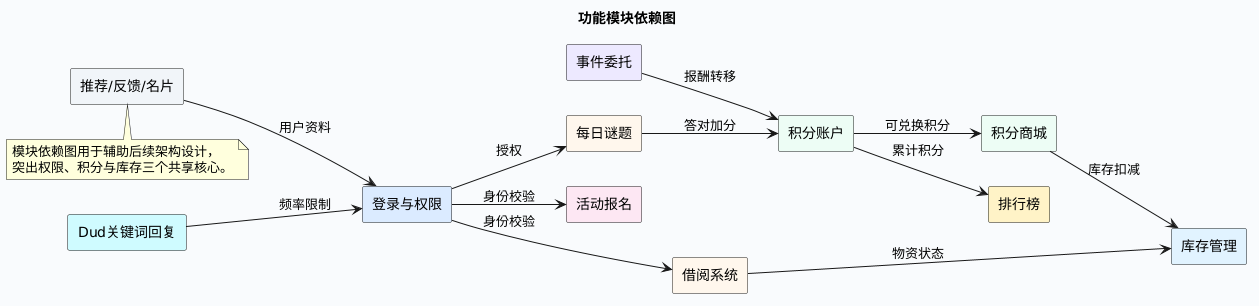
\includegraphics[width=0.86\textwidth,height=0.38\textheight,keepaspectratio]{uml_output/module_dependency.png}
    \caption{功能模块依赖图}
    \label{fig:module-dependency}
\end{figure}

如图 \ref{fig:module-dependency} 所示，系统的共享核心为登录与权限、积分账户和库存管理。每日谜题、排行榜、商城和事件委托依赖积分账户；借阅系统和商城依赖库存管理；活动、借阅、委托、反馈等操作均依赖登录与权限校验。该依赖关系要求后续设计中优先保证身份识别、积分流水和库存状态的一致性。

\section{非功能性需求}

\subsection{性能需求}
\begin{itemize}
    \item \textbf{响应延迟}：常规交互（如页面跳转、答题提交、消息回复）的系统响应时间必须控制在1.5秒至2秒以内。排行榜查询（涉及排序）允许最多3秒延迟。
    \item \textbf{高并发处理}：系统需能够支撑每日谜题更新点（通常为高峰期）至少50-100名用户同时发起查询或提交操作，且不产生数据锁冲突。云函数应配置适当的并发限制与超时时间（建议10秒）。
    \item \textbf{数据实时性}：排行榜数据需在每日谜题结算后实时更新（$\leq$ 1分钟），积分商城库存需在兑换成功后立即完成原子扣减（秒级同步）。
    \item \textbf{存储优化}：数据库查询应通过合理的索引策略优化，避免全表扫描；答题记录、借阅记录等大表应按时间分片存储。
\end{itemize}

\subsection{安全性需求}
\begin{itemize}
    \item \textbf{访问控制}：核心业务（每日谜题答题、活动报名、积分兑换、物品借阅、事件委托发布、个人名片修改等）必须经过微信授权登录并验证有效的session。未登录用户仅可浏览游戏与书籍推荐、公开活动通知、首页基础信息等不依赖 user\_id 的公开内容。后台管理入口需额外进行权限白名单校验，防止越权访问。
    \item \textbf{数据一致性}：在处理"事件委托"的积分转移或"借阅系统"的状态变更时，必须引入事务处理机制（ACID），确保积分不会凭空产生或消失。若发生中间状态异常，系统应能自动回滚。
    \item \textbf{业务防刷}：
        \begin{itemize}
            \item 每日谜题限制单一账号每日仅一次提交机会，前端与后端需双重校验。
            \item 关键词回复系统需限制频率（如单用户30秒内最多发送5条消息），防止刷屏。
            \item 库存扣减操作需使用数据库锁或CAS机制防止超额。
        \end{itemize}
    \item \textbf{信息隐私保护}：
        \begin{itemize}
            \item 用户的 OpenID（数据库字段为 \texttt{openid}）不应在客户端暴露或在日志中明文记录。
            \item 借阅记录中的个人隐私（如借阅时间、位置）仅对借阅人与管理员可见。
            \item 支持匿名反馈选项，系统不应泄露匿名反馈者身份。
        \end{itemize}
\end{itemize}

\subsection{可用性需求}
\begin{itemize}
    \item \textbf{UI/UX 设计}：
        \begin{itemize}
            \item 界面需体现侦探解谜风格，配合品牌色彩与图标（推荐采用Mystery/Detective主题配色）。
            \item 首页通过智能按钮颜色（如灰色代表已答，彩色代表待答）直观反馈用户当日任务状态。
            \item 排行榜中的用户头像应以不同背景色突出（如用户所在行采用浅高亮背景）。
        \end{itemize}
    \item \textbf{容错提示}：
        \begin{itemize}
            \item 对于逻辑限制操作（如在不可取消时间内尝试取消报名），系统必须通过强制性的弹窗反馈明确告知原因与后续操作建议。
            \item 网络超时、服务异常时，提示用户稍后重试，并记录操作日志便于排查。
        \end{itemize}
    \item \textbf{交互闭环}：
        \begin{itemize}
            \item 借阅逻辑中，借阅人需拥有专属的"取消"按钮，而第三方视图仅展示物资状态，确保权限与操作的一一对应。
            \item 用户发起任何积分交易（兑换、委托转账）都应获得即时的确认反馈与历史记录。
        \end{itemize}
    \item \textbf{无障碍设计}：支持屏幕阅读器，文字大小可调节，色彩对比度符合WCAG AA标准。
\end{itemize}

\subsection{可维护性与扩展性}
\begin{itemize}
    \item \textbf{配置灵活性}：
        \begin{itemize}
            \item Dud机器人的关键词库、每日谜题库应支持无需重新发布代码的热更新（通过数据库变更自动生效）。
            \item 管理员可在后台动态调整系统参数（如每日谜题更新时间、报名截止时间相对偏移等）。
        \end{itemize}
    \item \textbf{模块化架构}：系统各功能模块（如借阅、积分、报名）应解耦设计，形成清晰的内部接口与依赖图，便于未来扩展新的社团功能或更换更强大的云端引擎（如从云开发迁移至云服务器）。
    \item \textbf{代码与文档规范}：
        \begin{itemize}
            \item 采用统一的代码风格指南（如ESLint配置）与注释模板，保证代码可读性。
            \item 关键业务逻辑应配备设计文档与算法说明（如排行榜计算逻辑、借阅状态机等）。
        \end{itemize}
    \item \textbf{测试覆盖}：核心功能（如积分交易、权限校验）应拥有 $\geq$ 80\% 的单元测试覆盖率；关键业务流程应编写集成测试用例。
    \item \textbf{日志与监控}：
        \begin{itemize}
            \item 云函数应记录所有关键操作（如登录、积分变更、权限检查失败），便于事后审计与故障诊断。
            \item 建立性能监控仪表板，实时显示API响应时间、错误率、并发数等指标。
        \end{itemize}
\end{itemize}

\section{数据需求}

本系统的数据需求围绕微信小程序端的用户交互、社团物资流转、积分激励体系以及管理员后台维护展开。结合前文所述系统目标，本系统不仅是一个信息展示平台，还集成了每日谜题、积分排行、活动报名、物资借阅、积分兑换、关键词互动、个人名片和事件委托等模块。因此，系统数据既要支持普通用户在微信小程序端的实时操作，也要支持社团管理层在后台对谜题、活动、库存、规则和积分等核心数据进行维护。

由于系统运行环境以微信小程序云开发或自建云服务为主，用户身份识别应优先基于微信 OpenID，而不是传统的用户名密码登录。数据库可以采用微信云数据库中的集合形式进行存储，也可以在后续扩展为关系型数据库。无论采用何种底层数据库，本节均从逻辑数据模型角度描述系统所需的数据实体、实体关系和关键字段。

本章节是对前文第\ref{3}章节的补充和完善，主要依据小组成员绘制的类图\ref{fig:class-diagram}展开数据需求具体设计的描述。
\subsection{总体数据对象}

系统需要维护的主要数据对象包括用户信息、管理员权限信息、每日谜题信息、谜题选项信息、答题记录、积分账户、积分流水、排行榜快照、库存物品、兑换记录、活动信息、活动报名记录、反馈留言、剧本杀扩展信息、借阅记录、推荐内容、Dud 关键词回复规则、关键词对话日志、侦探个人名片、事件委托、委托接收记录、委托积分分配记录以及后台操作日志。

这些数据对象之间存在较强的业务关联。例如，每日谜题答题结果会影响用户积分；用户积分又影响排行榜和兑换商城；兑换商城中的商品库存与库存管理系统共享同一批库存数据；书籍和剧本杀的借阅状态也由库存管理系统统一维护；用户个人名片需要展示积分和排名；事件委托完成后会触发积分转移。因此，后续数据库设计必须保证各模块之间的数据来源一致，避免出现排行榜积分、可兑换积分、库存状态和个人页面展示数据相互矛盾的情况。

\subsection{用户与身份数据}

用户数据是所有业务操作的基础。由于系统部署为微信小程序，用户登录应以微信授权后的 OpenID 作为唯一身份标识。用户首次进入系统时，可以生成一条用户记录，并初始化其积分账户和个人名片。

用户信息数据项如下：

\begin{longtable}{p{3.5cm}p{3cm}p{7cm}}
\caption{用户信息数据项} \\
\toprule
字段名 & 数据类型 & 说明 \\
\midrule
user\_id & String & 系统内部用户唯一标识，可由云数据库自动生成 \\
openid & String & 微信用户唯一标识，用于登录和身份识别 \\
nickname & String & 用户昵称，默认可来自微信资料，也可由用户修改 \\
avatar\_url & String & 用户头像地址 \\
role & String & 用户角色，包括普通用户、管理员等 \\
status & String & 用户状态，包括正常、禁用、注销等 \\
created\_at & DateTime & 首次进入系统时间 \\
updated\_at & DateTime & 最近资料更新时间 \\
last\_login\_at & DateTime & 最近登录时间 \\
\bottomrule
\end{longtable}

其中，\texttt{openid} 是最重要的身份字段，必须保证唯一。普通用户只能操作与自身 \texttt{user\_id} 相关的数据；管理员则可以通过后台页面维护谜题、活动、库存、推荐内容、关键词规则和用户反馈等数据。管理员身份可以通过 \texttt{role} 字段控制，也可以单独建立管理员白名单集合，这样也符合前文安全性需求中“后台管理入口需额外进行权限白名单校验”的要求。

\subsection{个人名片数据}

侦探个人名片是用户个人页面的核心数据。个人名片既承担展示功能，也为后续帖子评论区、事件委托页面、排行榜页面等模块提供用户身份入口。用户注册后，系统应自动创建默认个人名片，用户之后可以自行修改交友信息和名片样式。

\begin{longtable}{p{3.5cm}p{3cm}p{7cm}}
\caption{侦探个人名片数据项} \\
\toprule
字段名 & 数据类型 & 说明 \\
\midrule
card\_id & String & 名片唯一标识 \\
user\_id & String & 所属用户编号 \\
display\_name & String & 名片显示名称 \\
campus & String & 所在校区 \\
grade & String & 年级，可选 \\
major & String & 专业，可选 \\
interests & Array/String & 兴趣标签，如推理小说、剧本杀、密室等 \\
self\_intro & String & 个人简介 \\
favorite\_works & Array/String & 喜欢的推理作品 \\
card\_style & Object & 名片样式配置，如背景、边框、主题色等 \\
visibility & String & 可见范围，如公开、仅社团成员可见、隐藏 \\
created\_at & DateTime & 创建时间 \\
updated\_at & DateTime & 最近修改时间 \\
\bottomrule
\end{longtable}

个人名片与用户是一对一关系。个人页面中显示的积分和排名不建议直接冗余存储在个人名片表中，而应从积分账户和排行榜数据中读取，以避免数据不同步。

\subsection{每日谜题数据}

每日谜题是首页的核心互动入口之一。根据前文系统范围，每日谜题应支持管理员预先设置，到点自动更新；首页不直接展示完整谜题内容，只通过按钮颜色提示用户今日是否已答题。进入谜题页面后，系统展示题干、选项、提交按钮、正确答案和解析。每个账号每天只能答题一次。

每日谜题数据由谜题主表、谜题选项和答题记录三部分组成。

\begin{longtable}{p{3.5cm}p{3cm}p{7cm}}
\caption{每日谜题数据项} \\
\toprule
字段名 & 数据类型 & 说明 \\
\midrule
puzzle\_id & String & 谜题唯一标识 \\
title & String & 谜题标题 \\
content & String & 谜题正文 \\
difficulty & String & 难度，如简单、中等、困难 \\
reward\_points & Number & 答对后获得的积分 \\
answer\_explanation & String & 答案解析 \\
publish\_date & Date & 对应日期 \\
publish\_time & DateTime & 定时发布时间 \\
status & String & 状态，包括草稿、待发布、已发布、已下线 \\
created\_by & String & 创建该谜题的管理员编号 \\
created\_at & DateTime & 创建时间 \\
updated\_at & DateTime & 更新时间 \\
\bottomrule
\end{longtable}

\begin{longtable}{p{3.5cm}p{3cm}p{7cm}}
\caption{谜题选项数据项} \\
\toprule
字段名 & 数据类型 & 说明 \\
\midrule
option\_id & String & 选项唯一标识 \\
puzzle\_id & String & 所属谜题编号 \\
option\_label & String & 选项标识，如 A、B、C、D \\
option\_content & String & 选项内容 \\
is\_correct & Boolean & 是否为正确答案 \\
sort\_order & Number & 选项显示顺序 \\
\bottomrule
\end{longtable}

\begin{longtable}{p{3.5cm}p{3cm}p{7cm}}
\caption{答题记录数据项} \\
\toprule
字段名 & 数据类型 & 说明 \\
\midrule
record\_id & String & 答题记录编号 \\
user\_id & String & 答题用户编号 \\
openid & String & 答题用户微信 OpenID \\
puzzle\_id & String & 谜题编号 \\
selected\_option\_id & String & 用户选择的选项编号 \\
is\_correct & Boolean & 是否回答正确 \\
score\_gained & Number & 本次获得积分 \\
answered\_at & DateTime & 答题时间 \\
\bottomrule
\end{longtable}

系统应对 \texttt{user\_id + puzzle\_id} 建立唯一约束，防止用户重复答题。答题成功后，系统应同时写入答题记录、更新积分账户，并生成积分流水。

\subsection{积分与排行榜数据}

积分体系分为两个逻辑维度：总累计积分和可兑换积分。总累计积分用于排行榜，体现用户历史贡献；可兑换积分用于商城消费和事件委托报酬，兑换或支付后会减少。两者不能混用，否则会导致排行榜和兑换商城的业务逻辑冲突。

\begin{longtable}{p{3.5cm}p{3cm}p{7cm}}
\caption{用户积分账户数据项} \\
\toprule
字段名 & 数据类型 & 说明 \\
\midrule
point\_account\_id & String & 积分账户编号 \\
user\_id & String & 所属用户编号 \\
total\_points & Number & 总累计积分，用于排行榜 \\
available\_points & Number & 可兑换积分，用于兑换商城和委托报酬 \\
frozen\_points & Number & 冻结积分，用于事件委托尚未结算的报酬 \\
used\_points & Number & 已消费积分 \\
updated\_at & DateTime & 最近更新时间 \\
\bottomrule
\end{longtable}

\begin{longtable}{p{3.5cm}p{3cm}p{7cm}}
\caption{积分流水数据项} \\
\toprule
字段名 & 数据类型 & 说明 \\
\midrule
transaction\_id & String & 积分流水编号 \\
user\_id & String & 用户编号 \\
change\_amount & Number & 积分变化值，可正可负 \\
point\_type & String & 积分类型，包括总积分、可兑换积分、冻结积分 \\
business\_type & String & 来源类型，如每日谜题、商城兑换、委托冻结、委托结算、管理员调整 \\
related\_id & String & 关联业务编号 \\
description & String & 流水说明 \\
created\_at & DateTime & 流水产生时间 \\
\bottomrule
\end{longtable}

排行榜数据可以采用“实时查询 + 每日快照”的方式处理。首页只展示前三名，因此可以直接读取最近一次排行榜快照中的前三项；完整排行榜页面展示前 100 名，并处理第 100 名同分扩展显示；个人中心则需要显示用户实时积分和实时排名。
\begin{longtable}{p{3.5cm}p{3cm}p{7cm}}
\caption{排行榜快照数据项} \\
\toprule
字段名 & 数据类型 & 说明 \\
\midrule
snapshot\_id & String & 快照编号 \\
ranking\_date & Date & 排行榜日期 \\
user\_id & String & 用户编号 \\
rank\_no & Number & 排名 \\
total\_points & Number & 快照生成时的总积分 \\
is\_top100 & Boolean & 是否属于前 100 名展示范围 \\
created\_at & DateTime & 快照生成时间 \\
\bottomrule
\end{longtable}
\subsection{库存、兑换与借阅数据}

库存管理系统是兑换商城和剧本杀/书籍借阅系统的共同数据基础。前文已经说明兑换奖品、书籍、剧本杀以及海报、办公用具等杂物都属于社团物资，因此应由统一的库存数据集合维护。不同业务模块只读取或修改同一份库存数据，避免出现商城库存与后台库存不一致的问题。

\begin{longtable}{p{3.5cm}p{3cm}p{7cm}}
\caption{库存物品数据项} \\
\toprule
字段名 & 数据类型 & 说明 \\
\midrule
item\_id & String & 物品编号 \\
item\_name & String & 物品名称 \\
item\_type & String & 物品类型，如书籍、剧本杀、兑换奖品、海报、办公用具 \\
description & String & 物品简介 \\
campus & String & 所在校区 \\
location & String & 具体存放位置 \\
total\_quantity & Number & 总数量 \\
available\_quantity & Number & 可用数量 \\
status & String & 状态，如在库、传递中、已借出、缺货、下架 \\
exchange\_points & Number & 兑换所需积分，仅兑换奖品使用 \\
cover\_url & String & 封面图片，可选 \\
created\_at & DateTime & 创建时间 \\
updated\_at & DateTime & 更新时间 \\
\bottomrule
\end{longtable}

剧本杀相比普通书籍需要额外记录类型、人数和游玩时长，因此设计扩展数据：

\begin{longtable}{p{3.5cm}p{3cm}p{7cm}}
\caption{剧本杀扩展数据项} \\
\toprule
字段名 & 数据类型 & 说明 \\
\midrule
script\_info\_id & String & 剧本杀扩展信息编号 \\
item\_id & String & 对应库存物品编号 \\
genre & String & 类型，如本格、变格、情感、机制等 \\
player\_min & Number & 最少游玩人数 \\
player\_max & Number & 最多游玩人数 \\
duration\_minutes & Number & 预计游玩时长 \\
difficulty & String & 难度，可选 \\
\bottomrule
\end{longtable}

兑换记录数据项如下：

\begin{longtable}{p{3.5cm}p{3cm}p{7cm}}
\caption{兑换记录数据项} \\
\toprule
字段名 & 数据类型 & 说明 \\
\midrule
exchange\_id & String & 兑换记录编号 \\
user\_id & String & 兑换用户编号 \\
item\_id & String & 兑换商品编号 \\
points\_cost & Number & 本次消耗的可兑换积分 \\
quantity & Number & 兑换数量 \\
status & String & 状态，如待领取、已完成、已取消 \\
created\_at & DateTime & 兑换时间 \\
handled\_by & String & 处理管理员编号 \\
handled\_at & DateTime & 处理时间 \\
\bottomrule
\end{longtable}

借阅记录数据项如下：

\begin{longtable}{p{3.5cm}p{3cm}p{7cm}}
\caption{借阅记录数据项} \\
\toprule
字段名 & 数据类型 & 说明 \\
\midrule
borrow\_id & String & 借阅记录编号 \\
item\_id & String & 借阅物品编号 \\
borrower\_id & String & 借阅用户编号 \\
status & String & 状态，包括在库、传递中、已借出、已归还、已取消等 \\
requested\_at & DateTime & 用户发起借阅时间 \\
lent\_at & DateTime & 管理员确认实物借出时间 \\
returned\_at & DateTime & 归还时间 \\
cancelled\_at & DateTime & 取消时间 \\
handled\_by & String & 后台处理管理员编号 \\
\bottomrule
\end{longtable}

当用户确认借阅后，库存物品状态应立即变为“传递中”。在“传递中”状态下，借阅人可以取消申请，其他用户只能看到该物品处于传递中，不能再次借阅。管理员实际交付物品后，再将状态改为“已借出”。

\subsection{活动与报名数据}

活动通知与报名模块需要支持活动展示、报名、取消报名、人数上限检查以及最晚取消时间判断。活动页面应按时间顺序展示近期活动，并实时显示是否报满。

\begin{longtable}{p{3.5cm}p{3cm}p{7cm}}
\caption{活动数据项} \\
\toprule
字段名 & 数据类型 & 说明 \\
\midrule
activity\_id & String & 活动编号 \\
title & String & 活动标题 \\
description & String & 活动简介 \\
start\_time & DateTime & 活动开始时间 \\
end\_time & DateTime & 活动结束时间 \\
location & String & 活动地点 \\
capacity & Number & 人数上限 \\
registered\_count & Number & 当前已报名人数，可由报名记录统计得到 \\
cancel\_deadline & DateTime & 最晚取消报名时间 \\
status & String & 活动状态，如报名中、已满、已结束、已取消 \\
created\_by & String & 创建管理员编号 \\
created\_at & DateTime & 创建时间 \\
updated\_at & DateTime & 更新时间 \\
\bottomrule
\end{longtable}

\begin{longtable}{p{3.5cm}p{3cm}p{7cm}}
\caption{活动报名记录数据项} \\
\toprule
字段名 & 数据类型 & 说明 \\
\midrule
registration\_id & String & 报名记录编号 \\
activity\_id & String & 活动编号 \\
user\_id & String & 报名用户编号 \\
status & String & 状态，如已报名、已取消 \\
registered\_at & DateTime & 报名时间 \\
cancelled\_at & DateTime & 取消时间 \\
can't\_cancel\_confirm & Boolean & 是否已确认“报名后不可取消”的提示 \\
\bottomrule
\end{longtable}

如果用户在最晚取消时间之后报名，系统应在提交前弹窗提示该活动报名后不可取消；用户确认后再生成报名记录。

\subsection{反馈留言数据}

活动申请、建议和问题反馈统一进入反馈留言模块。普通用户可以提交文本，管理员可以在后台查看、回复和处理。

\begin{longtable}{p{3.5cm}p{3cm}p{7cm}}
\caption{反馈留言数据项} \\
\toprule
字段名 & 数据类型 & 说明 \\
\midrule
feedback\_id & String & 留言编号 \\
user\_id & String & 提交用户编号 \\
feedback\_type & String & 类型，如活动建议、问题反馈、其他 \\
content & String & 留言内容 \\
is\_anonymous & Boolean & 是否匿名反馈 \\
status & String & 状态，如待处理、处理中、已处理 \\
reply & String & 管理员回复 \\
handled\_by & String & 处理管理员编号 \\
created\_at & DateTime & 提交时间 \\
handled\_at & DateTime & 处理时间 \\
\bottomrule
\end{longtable}

\subsection{推荐内容数据}

游戏/书籍推荐属于首页新闻通知的一部分。首页只展示入口或摘要，点击后进入独立推荐页面，用户可以上下翻阅全部推荐内容，并通过弹窗查看具体名称、类型、推荐人和推荐理由。

\begin{longtable}{p{3.5cm}p{3cm}p{7cm}}
\caption{推荐内容数据项} \\
\toprule
字段名 & 数据类型 & 说明 \\
\midrule
recommendation\_id & String & 推荐内容编号 \\
title & String & 游戏或书籍名称 \\
category & String & 推荐类型，如游戏、书籍、剧本杀 \\
genre & String & 作品类型 \\
recommender\_id & String & 推荐人编号，可为空 \\
reason & String & 推荐理由 \\
article\_url & String & 公众号文章链接，可为空 \\
cover\_url & String & 封面图地址 \\
status & String & 状态，如草稿、已发布、已下线 \\
published\_at & DateTime & 发布时间 \\
created\_at & DateTime & 创建时间 \\
updated\_at & DateTime & 更新时间 \\
\bottomrule
\end{longtable}

\subsection{Dud 关键词回复数据}

Dud 关键词回复系统对应首页的神秘按钮。用户进入独立对话界面后，系统根据管理员配置的关键词规则返回内容。规则需要支持多关键词全匹配、半匹配和优先级控制，并且应能通过后台热更新，不需要重新发布小程序代码。

\begin{longtable}{p{3.5cm}p{3cm}p{7cm}}
\caption{关键词回复规则数据项} \\
\toprule
字段名 & 数据类型 & 说明 \\
\midrule
rule\_id & String & 规则编号 \\
rule\_name & String & 规则名称 \\
match\_type & String & 匹配方式，如完全匹配、半匹配、多关键词全匹配 \\
keywords & Array & 关键词列表 \\
reply\_content & String & Dud 回复内容 \\
priority & Number & 匹配优先级，数值越高越优先 \\
is\_enabled & Boolean & 是否启用 \\
created\_by & String & 创建管理员编号 \\
created\_at & DateTime & 创建时间 \\
updated\_at & DateTime & 更新时间 \\
\bottomrule
\end{longtable}

\begin{longtable}{p{3.5cm}p{3cm}p{7cm}}
\caption{关键词对话日志数据项} \\
\toprule
字段名 & 数据类型 & 说明 \\
\midrule
chat\_log\_id & String & 对话日志编号 \\
user\_id & String & 用户编号，可为空 \\
input\_content & String & 用户输入内容 \\
matched\_rule\_id & String & 命中的规则编号，可为空 \\
reply\_content & String & 系统回复内容 \\
created\_at & DateTime & 对话时间 \\
\bottomrule
\end{longtable}

\subsection{事件委托数据}

事件委托模块类似社团内部求助或集市委托系统。用户可以发布求助帖，并以自身可兑换积分作为报酬。其他用户可以接收委托。委托完成后，发帖人确认事件解决，并将积分分配给接收委托的一个或多个用户。

另外，社团管理员也会定期发布任务，并且在社团发布的任务中，系统会自动将其置顶，确保它能够被优先看到。第一个完成任务的用户将获得积分。管理员可以发布委托任务，系统会根据任务的完成情况，按照发帖人设定的积分奖励进行积分分配。

\begin{longtable}{p{3.5cm}p{3cm}p{7cm}}
\caption{事件委托数据项} \\
\toprule
字段名 & 数据类型 & 说明 \\
\midrule
commission\_id & String & 委托编号 \\
publisher\_id & String & 发布用户编号 \\
title & String & 委托标题 \\
content & String & 委托内容 \\
reward\_points & Number & 设置的积分报酬 \\
status & String & 状态，如招募中、进行中、已解决、已关闭 \\
is\_pinned & Boolean & 是否置顶标志，表示该委托是否为社团发布的，默认置顶社团发布的委托 \\
created\_at & DateTime & 发布时间 \\
resolved\_at & DateTime & 解决时间 \\
\bottomrule
\end{longtable}

\begin{longtable}{p{3.5cm}p{3cm}p{7cm}}
\caption{委托接收记录数据项} \\
\toprule
字段名 & 数据类型 & 说明 \\
\midrule
acceptance\_id & String & 接收记录编号 \\
commission\_id & String & 委托编号 \\
receiver\_id & String & 接收委托的用户编号 \\
status & String & 状态，如已接收、已退出、已完成 \\
accepted\_at & DateTime & 接收时间 \\
completed\_at & DateTime & 完成时间 \\
\bottomrule
\end{longtable}

\begin{longtable}{p{3.5cm}p{3cm}p{7cm}}
\caption{委托积分分配数据项} \\
\toprule
字段名 & 数据类型 & 说明 \\
\midrule
allocation\_id & String & 分配记录编号 \\
commission\_id & String & 委托编号 \\
receiver\_id & String & 获得积分的用户编号 \\
allocated\_points & Number & 分配积分数 \\
created\_at & DateTime & 分配时间 \\
\bottomrule
\end{longtable}


\subsection{后台管理与操作日志数据}

管理员后台需要维护每日谜题、活动、库存、兑换商品、推荐内容、关键词回复规则和反馈留言。为保证数据可追溯，系统需要记录关键后台操作。

\begin{longtable}{p{3.5cm}p{3cm}p{7cm}}
\caption{后台操作日志数据项} \\
\toprule
字段名 & 数据类型 & 说明 \\
\midrule
log\_id & String & 日志编号 \\
admin\_id & String & 操作管理员编号 \\
operation\_type & String & 操作类型，如新增、修改、删除、上下架、状态变更 \\
target\_collection & String & 被操作的数据集合或数据表 \\
target\_id & String & 被操作记录编号 \\
before\_data & Object & 修改前数据快照 \\
after\_data & Object & 修改后数据快照 \\
created\_at & DateTime & 操作时间 \\
\bottomrule
\end{longtable}

后台操作日志尤其需要覆盖积分调整、库存调整、借阅状态变更、活动状态变更和关键词规则修改等关键操作。


\section{约束与假设}

\subsection{技术约束}

本系统的技术实现应与前文系统运行环境保持一致，即以微信小程序作为主要客户端，以微信 OpenID 作为用户身份识别依据，以云函数或后端接口作为业务逻辑层，以云数据库或等价数据库服务作为数据存储层。

\begin{enumerate}
    \item 系统前端必须运行在微信小程序环境中，页面结构、样式和逻辑应分别使用 WXML、WXSS 和 JavaScript/TypeScript 实现。
    \item 用户身份识别应基于微信授权登录后的 OpenID。系统不默认要求用户设置传统账号密码，除非后续引入独立 Web 后台或跨平台登录。
    \item 后端业务逻辑应通过云函数或自建后端 API 实现，客户端不得直接执行积分变更、库存扣减、排行榜更新等关键业务逻辑。
    \item 数据库可以采用微信云数据库集合，也可以采用自建数据库。若使用云数据库，应通过集合、文档、索引和事务能力实现本报告中的逻辑数据模型。
    \item 每日谜题发布、排行榜快照生成、过期活动状态更新等任务需要定时执行。若使用微信云开发，应通过定时触发器或云函数实现。
    \item 积分兑换、库存扣减、借阅状态修改、委托积分冻结与转移等操作必须通过数据库事务或等价的原子操作完成。
    \item 后台管理功能必须进行管理员权限校验，不能仅依赖前端隐藏入口。
    \item 系统应与前文非功能性需求中的响应时间要求一致：普通页面跳转和提交操作应尽量控制在 1.5 至 2 秒内，排行榜查询可适当放宽但不应超过 3 秒。
    \item 对于首页、排行榜、推荐内容等高频读取数据，可以采用缓存或预计算方式优化，但缓存数据必须与数据库最终一致。
    \item 所有涉及用户输入的文本，如反馈留言、个人简介、委托内容和关键词输入，都需要进行内容长度限制和必要的安全过滤。
\end{enumerate}

\subsection{业务约束}

业务约束必须与前文需求保持一致，这里总结概括一些关键点，包括：

\begin{enumerate}
    \item 未登录用户可以浏览部分公开内容（如游戏与书籍推荐内容、公开活动通知与活动列表信息、小程序首页基础展示信息），但不能参与每日谜题答题、活动报名、积分兑换、物品借阅、事件委托发布、个人名片修改等操作。
    \item 每个用户每天只能回答一次每日谜题。后端必须根据 \texttt{user\_id} 和 \texttt{puzzle\_id} 进行重复提交校验。
    \item 用户提交每日谜题答案后，无论回答正确与否，都应显示正确答案和解析。
    \item 用户答对每日谜题后，系统应增加其积分，并同步生成积分流水。
    \item 总累计积分用于排行榜，可兑换积分用于商城兑换和事件委托，两者必须分开记录。
    \item 用户兑换奖品时，只扣除可兑换积分，不扣除总累计积分。
    \item 商城可兑换奖品的库存必须与库存管理系统共用同一份库存数据。
    \item 首页排行榜只展示前三名；完整排行榜默认展示前 100 名。
    \item 若第 100 名存在同分用户，应额外显示这些同分用户，避免同分情况下排名展示不公平。
    \item 用户个人页面应显示实时积分和排名；如果用户未进入排行榜前 100 名，则显示“未入榜”。
    \item 活动页面应按时间顺序展示近期活动，活动信息至少包括标题、简介、时间、地点、人数上限和是否报满。
    \item 用户对同一活动只能存在一条有效报名记录，不能重复报名。
    \item 活动报名人数不能超过人数上限。
    \item 用户只能在最晚取消时间之前取消报名。
    \item 若用户在最晚取消时间之后报名，系统必须在报名提交前弹窗提示报名后不可取消。
    \item 书籍和剧本杀只有在“在库”状态下才能被申请借阅。
    \item 用户确认借阅后，物品状态立即变为“传递中”。
    \item 物品处于“传递中”状态时，只有借阅申请人可以取消申请，其他用户不能借阅该物品。
    \item 管理员实际交付物品后，才可以将物品状态从“传递中”改为“已借出”。
    \item 物品归还后，管理员应将状态改为“在库”，并更新借阅记录。
    \item 反馈留言提交后，普通用户只能查看自己的反馈，管理员可以查看全部反馈。
    \item Dud 关键词回复规则只能由管理员维护，普通用户不能修改规则。
    \item 当多条关键词规则同时命中时，系统应根据优先级返回回复内容。
    \item 用户发布事件委托时，必须拥有足够可兑换积分作为报酬。
    \item 委托发布后，对应积分应进入冻结状态，防止用户在委托完成前消费该部分积分。
    \item 委托完成后，只有发帖人可以确认事件解决并分配积分。
    \item 委托积分分配总额不得超过发布委托时冻结的积分报酬。
\end{enumerate}

\subsection{数据完整性约束}

为了保证各模块数据不互相矛盾，系统需要满足以下数据完整性约束：

\begin{enumerate}
    \item 所有核心数据对象必须具有唯一编号。
    \item 用户的 \texttt{openid} 必须唯一。
    \item 每个用户只能拥有一个有效积分账户。
    \item 每个用户只能拥有一张当前有效的侦探个人名片。
    \item 每个用户对同一每日谜题只能有一条答题记录。
    \item 每个用户对同一活动只能有一条当前有效报名记录。
    \item 库存总数、可用数量、积分数、报名人数上限等数值字段不得为负数。
    \item 库存可用数量不得大于库存总数量。
    \item 活动已报名人数不得大于活动人数上限。
    \item 用户可兑换积分不得小于 0。
    \item 用户冻结积分不得小于 0。
    \item 用户用于委托的冻结积分不得超过其可兑换积分。
    \item 兑换记录中的 \texttt{points\_cost} 应保存兑换发生时的积分价格，不能因后续商品价格调整而改变。
    \item 积分流水原则上只允许追加，不允许直接删除或覆盖。若出现错误，应通过反向流水进行修正。
    \item 已经产生答题记录的每日谜题不应随意修改正确答案；如必须修改，应记录后台操作日志。
    \item 已经产生兑换或借阅记录的库存物品不应直接物理删除，应采用下架或停用状态。
    \item 后台操作日志一经生成，不应被普通管理员随意删除。
\end{enumerate}

\subsection{安全与隐私约束}

系统需要保护用户身份信息、个人名片信息、积分记录、活动报名记录和借阅记录。安全约束如下：

\begin{enumerate}
    \item 用户 OpenID 不应在小程序前端页面中直接暴露。
    \item 普通用户不能访问后台管理页面和后台管理接口。
    \item 管理员权限必须在服务端校验，不能只依赖前端判断。
    \item 普通用户不得查看其他用户的敏感信息，如 OpenID、联系方式、借阅历史等。
    \item 个人名片应支持可见范围设置。
    \item 积分流水、兑换记录、借阅记录和活动报名记录应只允许本人和管理员查看。
    \item 匿名反馈不得向普通用户暴露提交者身份。
    \item 用户输入内容应进行安全过滤，防止脚本注入、恶意链接和异常长文本。
    \item 对高频操作如关键词对话、重复提交答题、频繁刷新排行榜等，应设置合理的频率限制。
    \item 管理员进行积分调整、库存修改、借阅状态变更等关键操作时，应写入后台操作日志。
\end{enumerate}

\subsection{性能与并发约束}

结合前文非功能性需求，系统需要满足以下性能和并发约束：

\begin{enumerate}
    \item 首页应只加载必要摘要数据，包括每日谜题入口状态、排行榜前三名和推荐入口，避免一次性加载完整业务数据。
    \item 每日谜题提交、活动报名、商城兑换和借阅申请应尽量在 2 秒内完成反馈。
    \item 排行榜查询涉及排序，允许比普通页面略慢，但应通过索引、快照或缓存控制在 3 秒以内。
    \item 每日谜题更新点可能出现集中访问，系统应支持至少 50 至 100 名用户同时查询或提交。
    \item 商城兑换和活动报名必须处理并发场景，防止库存超卖和报名人数超过上限。
    \item 借阅申请必须处理并发场景，防止多个用户同时借阅同一本书或同一个剧本杀。
    \item 推荐内容、活动列表、借阅列表和委托列表应支持分页或滚动加载。
    \item 库存管理后台应支持按物品类型、校区、状态和关键词筛选。
    \item 关键词回复规则应按启用状态、优先级和关键词建立合理索引，保证 Dud 对话界面响应及时。
\end{enumerate}

\subsection{环境与部署假设}

在当前需求文档阶段，系统设计基于以下环境假设：

\begin{enumerate}
    \item 系统主要运行在微信小程序环境中，用户通过微信客户端访问。
    \item 系统优先使用微信 OpenID 识别用户身份。
    \item 系统初期不要求用户设置独立账号密码。
    \item 系统初期采用微信云开发或等价云服务，后续可迁移至自建服务器。
    \item 数据存储可以使用云数据库集合；本报告中的“表”和“字段”均表示逻辑数据结构，不限定物理数据库必须为关系型数据库。
    \item 社团管理层通过小程序内管理页面或独立后台页面进行数据维护。
    \item 系统初期不接入在线支付、物流配送和校园统一身份认证。
    \item 兑换奖品和借阅物品的实际交付主要在线下完成，系统负责记录状态和提供管理依据。
\end{enumerate}

\subsection{业务假设}

除技术环境外，系统业务流程还基于以下假设：

\begin{enumerate}
    \item 系统主要服务于 NK 推理协会内部成员和关注社团活动的普通用户，整体用户规模为中小型社团规模。
    \item 每日谜题默认每天发布一道，由管理员提前录入并设置发布时间。
    \item 每日谜题初期以单选题为主，但数据结构允许扩展为多选题。
    \item 答题奖励积分由管理员在创建谜题时设置。
    \item 排行榜按照总累计积分降序排列；积分相同则允许并列排名。
    \item 可兑换积分的来源包括每日谜题奖励、事件委托奖励和管理员手动调整。
    \item 兑换商品以线下领取为主，因此兑换状态需要管理员处理。
    \item 活动报名初期采用先到先得机制，不默认启用候补队列。
    \item 借阅物品一次只能被一个用户申请或借出。
    \item 剧本杀和书籍借阅仍由线下完成交付，系统负责申请、状态流转和记录。
    \item 推荐内容由管理员统一发布，普通用户可以作为推荐人出现在推荐信息中。
    \item Dud 关键词回复以规则匹配为主，不引入复杂自然语言理解模型。
    \item 事件委托中的积分由发帖人自行设置，系统负责冻结、转移和记录。
\end{enumerate}

\subsection{扩展假设}

为保证系统后续可扩展，当前设计保留以下扩展空间：

\begin{enumerate}
    \item 后续可以接入校园统一身份认证，实现用户身份与学校信息绑定。
    \item 活动报名可以增加候补机制和自动通知机制。
    \item 借阅系统可以增加归还提醒和逾期提醒。
    \item 积分体系可以增加限时积分、活动积分或积分有效期。
    \item 推荐内容和事件委托可以增加评论、点赞、收藏功能。
    \item 后台可以增加统计报表，包括活动参与率、谜题答对率、热门借阅物品、积分分布和关键词命中率。
    \item Dud 关键词回复系统后续可以扩展为更复杂的剧情式解谜系统。
\end{enumerate}


\end{document}
